\documentclass[12pt, a4paper]{article}

\usepackage[utf8]{inputenc}
% Limit the page margin to only 1 inch.
\usepackage[margin=1in]{geometry}

%Imports biblatex package
\usepackage[
backend=biber,
style=alphabetic
]{biblatex}
\addbibresource{../../algs4e.bib}

% Enables the `align' environment.
\usepackage{amsmath}
% Provides useful environments, such as:
% - \begin{proof} ...\end{proof}
\usepackage{amsthm}
\usepackage[most]{tcolorbox}

\newtheorem*{proposition}{Proposition}

% Enables using \mathbb{}, for example \mathbb{N} for the set of natural numbers.
\usepackage{amssymb}

% Allows using letters in enumerate list environment. Use, for example:
%\begin{enumerate}[label=(\alph*)]
% ...
%\end{enumerate}
\usepackage[inline]{enumitem}

% Enable importing external graphic files and provides useful commannds, like \graphicspath{}
\usepackage{graphicx}
% Images are located in a directory called images in the current directory.
\graphicspath{{./images/}}

% Make links look better by default.
% See: https://tex.stackexchange.com/questions/823/remove-ugly-borders-around-clickable-cross-references-and-hyperlinks
\usepackage[hidelinks]{hyperref}
\usepackage{xcolor}
\hypersetup{
	colorlinks,
	linkcolor={red!50!black},
	citecolor={blue!50!black},
	urlcolor={blue!80!black}
}


% Code Listings. Source:
% https://stackoverflow.com/questions/3175105/inserting-code-in-this-latex-document-with-indentation
\usepackage{listings}
\usepackage{color}

\definecolor{dkgreen}{rgb}{0,0.6,0}
\definecolor{gray}{rgb}{0.5,0.5,0.5}
\definecolor{mauve}{rgb}{0.58,0,0.82}

\lstset{frame=tb,
	language=Java,
	aboveskip=3mm,
	belowskip=3mm,
	showstringspaces=false,
	columns=flexible,
	basicstyle={\small\ttfamily},
	numbers=none,
	numberstyle=\tiny\color{gray},
	keywordstyle=\color{blue},
	commentstyle=\color{dkgreen},
	stringstyle=\color{mauve},
	breaklines=true,
	breakatwhitespace=true,
	tabsize=3
}

\newcommand{\prob}{\text{P}}
%\newcommand{\complement}{\mathsf{c}}

% Define an environment called "ex" (for Exercise) so that I can do: \begin{ex}{1.5}...\end{ex}
\newenvironment{ex}[2][Exercise]
{\par\medskip\noindent \textbf{#1 #2.}}
{\medskip}

% Define a solution environment, similar to ex (exercise) environment.
\newenvironment{sol}[1][Solution]
{\par\medskip\noindent \textbf{#1.} }
{\medskip}

\begin{document}
	\noindent Sergio E. Garcia Tapia \hfill
	
	\noindent \emph{Algorithms} by Sedgewick and Wayne (4th edition) \cite{sedgewick_wayne}\hfill
	
	\noindent November 2nd, 2024\hfill 
	\section*{2.4: Priority Queues}
	\begin{ex}{1}
		Suppose that the sequence \texttt{P R I O * R * * I * T * Y * * * Q U E * * * U * E}
		(where a letter means \emph{insert} and an asterisk means \emph{remove the maximum})
		is applied to an initially empty priority queue. Give the sequence of letters
		returned by the \emph{remove the maximum} operations.
	\end{ex}
	\begin{sol}
		\begin{lstlisting}[language={}]
P
P R
P R I
P R I O
P I O // max removed: R
P I O R
P I O // max removed: R
I O // max removed: P
I O I
I I // max removed: O
I I T
I I // max removed: T
I I Y
I I // max removed: Y
I // max removed: I
// max removed: I
Q
Q U
Q U E
Q E // max removed:  U
E // max removed: Q
// max removed: E
U
// max removed: U
E
		\end{lstlisting}
		At the end, \texttt{E} remains on the queue. The sequence letters returned is:
		\begin{center}
			\texttt{R R P O T Y I I U Q E U}
		\end{center}
	\end{sol}
	\begin{ex}{2}
		Criticize the following idea: To implement \emph{find the maximum} in constant
		time, why not use a stack  or a queue, but keep track of the maximum value inserted
		so far, then return that value for \emph{find the maximum}.
	\end{ex}
	\begin{sol}
		One issue is that this only guarantees that the first \emph{find the maximum}
		operation can be returned in constant time. Once that items is removed, if the client
		then asks for the next value, this operation then requires linear time.
	\end{sol}
	\begin{ex}{3}
		Provide priority-queue implementations that support \emph{insert} and
		\emph{remove the maximum}, one for each of the following underlying data structures:
		unordered array, ordered array, unordered linked list, and ordered linked list.
		Give a table of the worst-case bounds for each operation for each of your
		four implementations.
	\end{ex}
	\begin{sol}
		See package \texttt{com.segarciat.algs4.ch2.sec4.ex03}. The time complexities
		for the two main operations are given below for priority queue with $n$ items:
		\begin{center}
			\begin{tabular}{c|c|c}
				{} & Insert & Remove the maximum\\
				\hline
				\texttt{UnorderedArrayMaxPQ} & $O(1)$ & $O(n)$ \\
				\hline
				\texttt{OrderedArrayMaxPQ} & $O(n)$ & $O(1)$\\
				\hline
				\texttt{UnorderedListMaxPQ} & $O(1)$ & $O(n)$ \\
				\hline
				\texttt{OrderedListMaxPQ} & $O(n)$ & $O(1)$
			\end{tabular}
		\end{center}
	\end{sol}
	\begin{ex}{4}
		Is an  array that is sorted in decreasing order a max-oriented heap?
	\end{ex}
	\begin{sol}
		If we take entry \texttt{a[k]}, then it will certainly be larger than
		\texttt{a[2*k]} and \texttt{a[2*k + 1]}. Therefore if we see it as a
		binary tree, the binary tree is heap-ordered. In short, yes it is.
	\end{sol}
	\begin{ex}{5}
		Give the heap that results when the keys \texttt{E A S Y Q U E S T I O N}
		are inserted in that ordered into an initially empty max-oriented heap.
	\end{ex}
	\begin{sol}
		See Figure~\ref{fig:ex-05}.
		\begin{figure}
			\centering
			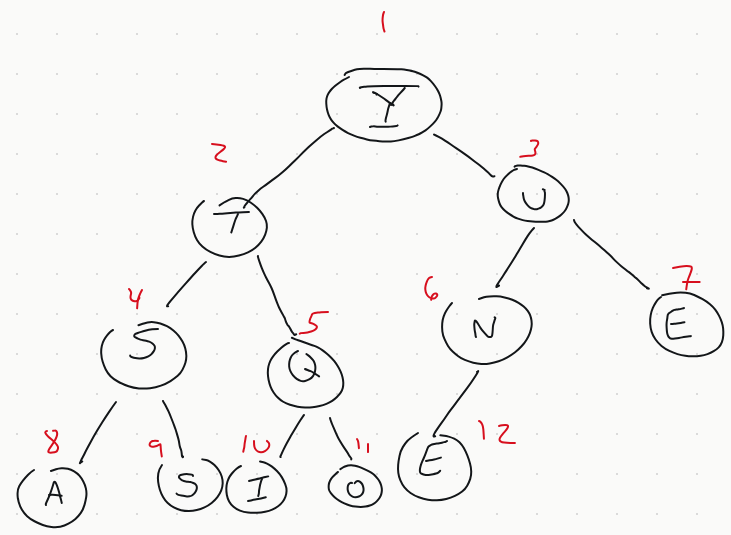
\includegraphics[width=0.6\textwidth]{exercise-05}
			\caption{Priority queue built out of keys \texttt{E A S Y Q U E S T I O N}
				for Exercise 2.4.5}
			\label{fig:ex-05}
		\end{figure}
		
		The contents of the corresponding array would be:
		\begin{lstlisting}[language={}]
[ null, "Y", "T", "U", "S", "Q", "N", "E", "A", "S", "I", "O", "E" ]
		\end{lstlisting}
	\end{sol}
	\begin{ex}{6}
		Using the conventions of Exercise 2.4.1, give the sequence of heaps produced
		when the operations \texttt{P R I O * R * * I * T * Y * * * Q U E * * * U * E} are
		performed on an initially empty max-oriented heap.
	\end{ex}
	\begin{sol}
		\begin{figure}
			\centering
			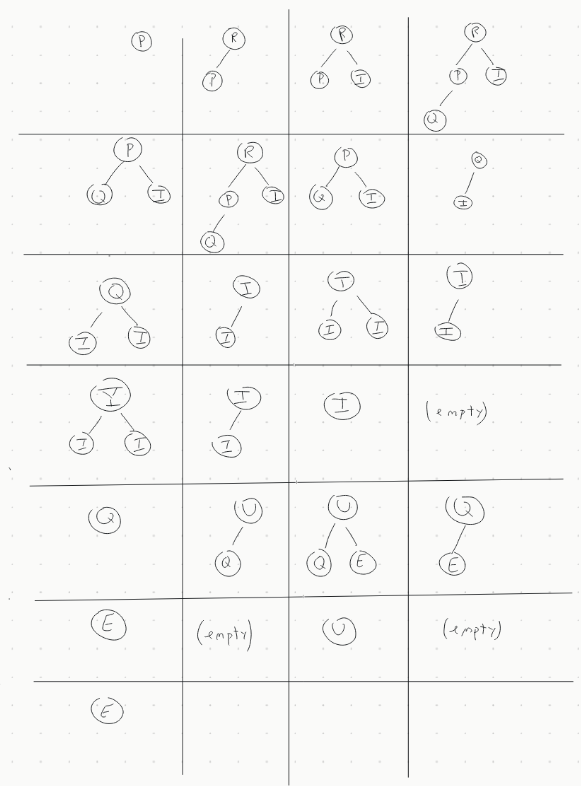
\includegraphics[width=0.9\textwidth]{exercise-06}
			\caption{Sequence of priority queue for Exercise 2.4.6}
			\label{fig:ex-06}
		\end{figure}
		See Figure~\ref{fig:ex-06}.
	\end{sol}
	\begin{ex}{7}
		The largest item in a heap must appear in position \texttt{1}, and the second
		largest must be in position \texttt{2} or \texttt{3}. Give the list of positions
		in a heap of size 31 where the $k$th largest:
		\begin{enumerate}[label=(\roman*)]
			\item can appear, and
			\item cannot appear,
		\end{enumerate}
		for $k=2,3,4$  (assuming the values to be distinct).
	\end{ex}
	\begin{sol}
		\begin{enumerate}[label=(\roman*)]
			\item Interpreting $k$ to start at $0$, where $0$th largest means largest,
			$1$th largest means 2nd largest, now we are considering $k=2$, which
			is the third largest.
			\begin{itemize}
				\item $k=2$ (third largest): Position 1 is taken by the largest. The second largest
				is at position 2 or position 3. The third largest could be at position 2
				or 3 as well (whichever one is not occupied by the second largest).
				In this case, it would be a child of the largest. Otherwise, it could
				be a child of the second largest. If the second largest is at position 2
				and the third largest was it child, then it could be at positions
				4 or 5. If the second largest is at position 3 and the third largest is
				its child, the it could be at position 6 or 7.
				
				Altogether, third largest could be in positions $\{2,3,4,5,6,7\}$.
				
				\item $k=3$ (fourth largest): This item could be a child of the largest,
				allowing for it to be at positions 2 or 3. This happens if the third
				largest is a child of the second largest.
				
				
				If the fourth largest is not a child of the largest, it could be a child of
				the second largest. Hence this would allow for positions 4, 5, 6, 7. Instead, if
				the fourth largest was a child of the third largest, then we have a few
				cases. If the 3rd largest was at positions 2 and 3, then we get no new
				information, since that would suggest positions 4,5,6,7 for the fourth
				largest, which we already know.
				
				However, the third largest may also be at positions $4,5,6,7$. If the the
				fourth largest is a child of the third, then it could be at a position that
				is a child of those positions. These are $8,9,10,11,12,13,14,15$.
				
				Hence, the fourth largest may appear at positions numbered in
				\[
				\{2,3,4,5,6,7,8,9,10,11,12,13,14,15\}
				\]
				
				
				\item $k=4$ (fifth largest): The fifth largest could be at positions
				2 and 3. Again, this would, for example if the second largest is at position
				2, and the third and fourth largest are its children.
				
				Similarly, the fifth largest could be at positions 4,5,6,7. This could
				happen, for example, if the second and third largest fill up positions
				2 and 3.
				
				Next, if the second and third largest fill up positions 2 and 3, and
				if the fourth largest fills up one of the positions 4,5,6,7, then
				by making the fifth largest a child of the fourth largest, we could
				have it fill positions $8,9,10,11,12,13,14,15$.
				
				One last possibility is if the second is a child of the first, the
				third is a child of the second, and the fourth is a child of the third.
				If we now make the fifth largest a child of the fourth, then it
				could take on any integer position between $16$ and $31$, inclusive.
				
				Hence, the fifth largest could be anywhere between positions 2 and 31,
				inclusive.
			\end{itemize}
			\item The places they may not appear are precisely the complement
			of the locations I found.
		\end{enumerate}
	\end{sol}
	\begin{ex}{8}
		Answer the previous exercise for the $k$th \emph{smallest} item.
	\end{ex}
	\begin{sol}
		Consider first where the smallest may be. The smallest cannot have a child.
		Thus  it must be in positions $16$ through $31$, inclusive. The second smallest
		must also be at positions $16$ through $31$ because even though it may have the
		smallest key as its child, it cannot have any other key as its child.
		Since the tree has $31$ nodes, it is a perfect tree, so every internal node
		has two children. Since the second smallest cannot have two children,
		it follows that it cannot be an internal node.
		\begin{enumerate}[label=(\roman*)]
			\item \begin{itemize}
				\item $k=2$ (third smallest): The third smallest may be in any of
				positions $16$ through $31$ as before. Since it can have the smallest
				and second smallest as its children, it could also be at positions
				$8$ through $15$. It cannot be at a higher level because that would
				imply that it is the root of a binary tree with 7 nodes, making it
				larger than 6 other nodes, and that's not the case.
				\item $k=3$ (fourth smallest): By a similar reasoning as $k=2$,
				it can only be at positions $8$ through $31$.
				\item $k=4$ (fifth smallest): By a similar reasoning as $k=2$,
				it can only be at positions $8$ through $31$. For example if it
				was at position $7$, then its two children and their children would
				all be smaller. This is impossible since the fifth smallest can only
				be larger than four other keys, not six.
			\end{itemize}
			\item Again just take the complements of the positions previous found.
		\end{enumerate}
	\end{sol}
	\begin{ex}{9}
		Draw all of the different heaps that can be made from the five keys
		\texttt{A B C D E}, then draw all of the different heaps that can be made from
		the five keys \texttt{A A A B B}.
	\end{ex}
	\begin{sol}
		I made the heaps max-oriented. See Figure~\ref{fig:ex-09-no-duplicates}
		and Figure~\ref{fig:ex-09-duplicates}.
		\begin{figure}
			\centering
			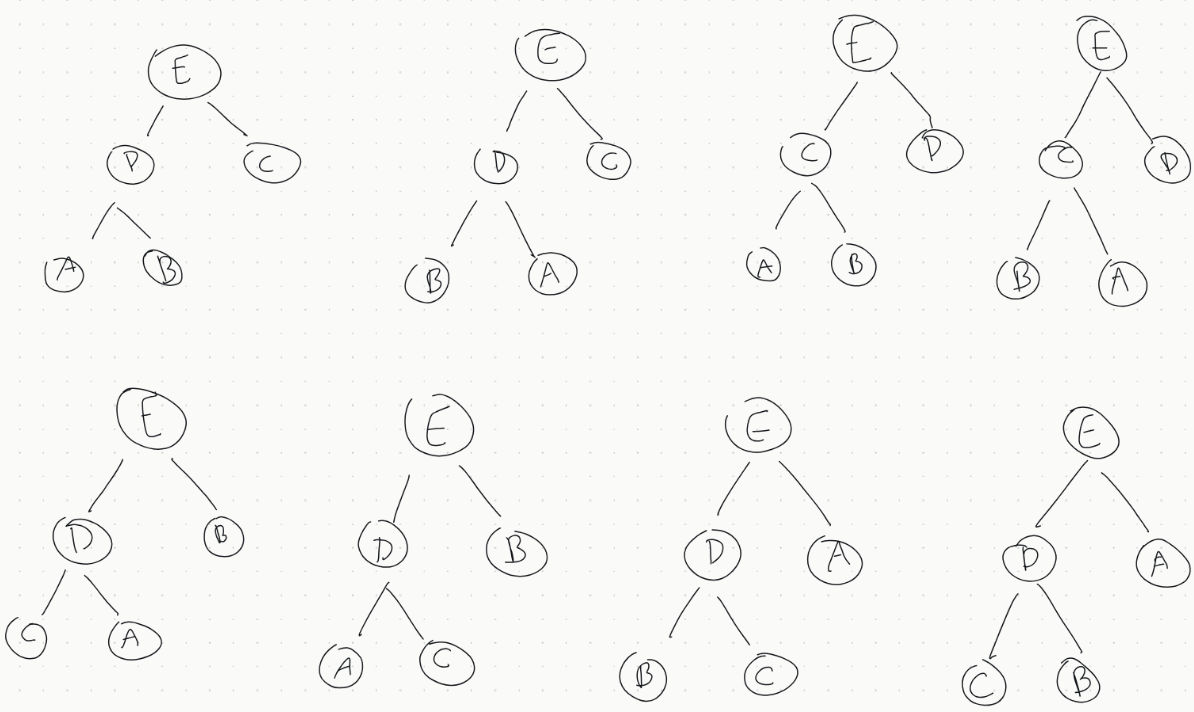
\includegraphics[width=0.8\textwidth]{exercise-09-no-duplicates}
			\caption{Exercise 2.4.9: All possible max-oriented heap with keys \texttt{A, B, C, D, E}}
			\label{fig:ex-09-no-duplicates}
		\end{figure}
		\begin{figure}
			\centering
			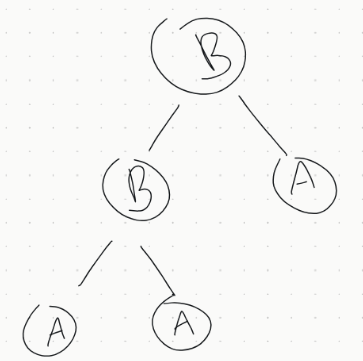
\includegraphics[width=0.3\textwidth]{exercise-09-duplicates}
			\caption{Exercise 2.4.9: All possible max-oriented heap with keys \texttt{A, A, A, B, B}}
			\label{fig:ex-09-duplicates}
		\end{figure}
	\end{sol}
	\begin{ex}{10}
		Suppose that we wish to avoid wasting one position in a heap-ordered array
		\texttt{pq[]}, putting the largest value in \texttt{pq[0]}, its children in
		\texttt{pq[1]} and \texttt{pq[2]}, and so forth, proceeding in level order.
		Where are the parents and children of \texttt{pq[k]}?
	\end{ex}
	\begin{sol}
		The children are at position $2k+1$ and $2k+2$. The parent is at $\lfloor \frac{k-1}{2}\rfloor$.
	\end{sol}
	\begin{ex}{11}
		Suppose that your application will have a huge number of \emph{insert} operations,
		but only a few \emph{remove the maximum} operations. Which priority-queue implementation
		do you think would be most effective: heap, unordered array, or ordered array?
	\end{ex}
	\begin{sol}
		The worst would be the ordered array implementation because it's expensive
		to add an item, given that it must maintain the keys in order.
		
		On the one hand, the unordered array implementation seems right for the job
		because inserts are $O(1)$, even though remove operations are $O(n)$.
	\end{sol}
	\begin{ex}{12}
		Suppose that your application will have a huge number of \emph{find the maximum}
		operations, but a relatively small number of \emph{insert} and \emph{remove the maximum}
		operations. Which priority-queue implementation do you think would be most effective:
		heap, unordered array, or ordered array?
	\end{ex}
	\begin{sol}
		The ordered appear implementation requires $O(1)$ for find-the-maximum operations.
		Even though inserts take $O(n)$, this seems like the best tool for the job.
	\end{sol}
	\begin{ex}{13}
		Describe a way to avoid the \texttt{j < n} test in \texttt{sink()}.
	\end{ex}
	\begin{sol}
		The context in which this test appears is that we are checking to see
		whether a node is smaller than its largest child. However the largest
		child could be the right child, and that child could be the last node
		in the heap. The way the code was presented, not having this test means
		we could have an \texttt{IndexOutOfBoundsException}.
		
		Since this can only happen at the last level, we could eliminate the
		test altogether, but change the controlling expression of the \texttt{while}
		from \texttt{2*k <= n} to \texttt{2*k < n}. This way, we guarantee that
		\texttt{2*k + 1 <= n}, so that \texttt{less(2k, 2k + 1)} is also valid.
		
		Now if the loop breaks ends because of the \texttt{while} controlling
		expression is \texttt{false}, then we know that \texttt{2 * k == n}.
		Thus, we can add an \texttt{if}, statement after the loop to check
		for this condition, and if the key at \texttt{k} is smaller than
		the key at \texttt{2 * k} (which equals \texttt{n}), then we do the
		final exchange.
		
		Alternatively, we can check if \texttt{n} is even, because only in this
		case can we have this issue. If so, we can exchange the item at position
		\texttt{k} and the item at position \texttt{n}, if \texttt{a[k] < a[n]}.
		Then once again we change the \texttt{while} controlling expression to
		\texttt{2*k <= n} to \texttt{2*k < n}. Now the test \texttt{j < n}
		can be eliminated.
	\end{sol}
	\begin{ex}{14}
		What is the minimum number of items that must be exchanged during a
		\emph{remove the maximum} operation in a heap of size $n$ with no duplicate keys?
		Give a heap of size $15$ for which the minimum is achieved. Answer the same
		questions for two and three successive \emph{remove the maximum} operations.
	\end{ex}
	\begin{sol}
		Suppose the heap has a single child at the last level, which can occur
		if $n=2^k$ for some integer $k$. The height of such a tree is $k$. In
		a max-oriented binary heap, the root contains the largest key. When
		a \emph{remove the maximum} operation is issued, the root is exchanged
		with the last node in the tree, and the new root now sinks through the
		heap until the correct location for it is found. The number of exchanges
		is dependent on the value of the key of that last node, but it must
		be at most $k-1$ because the tree decreases in height in this instance.
		
		Suppose the last node is the $(k+1)$th largest key, where the $0$th largest
		key is the largest key in the heap (located at the root). This could happen,
		for example, if the second and third largest are children of the root, and
		all next largest  nodes are under the subheap rooted at the third largest.
		For example, the fourth largest is a child of the third largest, the fifth
		largest is a child of the fourth, and so on. Since the height of the
		tree is $k$, this allows the $n$th node to be the $(k+1)$th largest.
		In particular, no node in the subheap rooted at the second largest key
		is larger than the last node. When the \emph{remove the maximum operation}
		is issued, the last node becomes the root and then sinks.  Since the second
		largest was a child of the old root, the exchange happens in that direction,
		so at least 1 exchange happens. However, no more exchange happens, because
		no node in the subheap that was rooted at the second largest (which is now
		the largest) was larger than the old $(k+1)$th largest node (now the $k$th
		largest node). The conclusion is that only 2 were required; the initial exchange
		with the old root, and the exchange between the old $(k+1)$th largest
		and old second largest!
		
		If the tree has size $n$ and height $k=\lfloor n\rfloor$, with $k\neq 2^k$,
		then a similar argument once again shows that only one exchange is necessary.
		See Figure~\ref{fig:ex-14-remove-max-once}.
		\begin{figure}
			\centering
			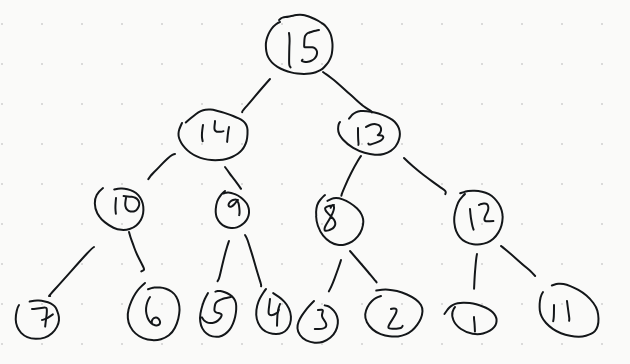
\includegraphics[width=0.5\textwidth]{exercise-14-remove-max-once}
			\caption{Exercise 14: Heap for which the first \emph{remove the maximum} operation
			would require 2 exchanges.}
			\label{fig:ex-14-remove-max-once}
		\end{figure}
		
		A similar setup leads to a minimum of 6 exchanges when 2 \emph{remove the maximum}
		operations are issued one after the other. This time, assume $n\neq 2^k$,
		Suppose that the tree has size $n$ with height $k=\lfloor \lg n\rfloor$,
		and $n\neq 2^k$. By a similar vein, have the largest at the root, the second
		and largest as its child. However, this time we make the third largest
		a child of the second. The other child of the root will be the fourth
		largest, which in turn is the parent of the fifth largest, and so on.
		Now the leaf becomes the $(k+2)$th largest instead of the $(k+1)$th as before.
		Its sibling is the $(k+3)$th largest, and both are children of the $k$th
		largest. When the first \emph{remove the max} operation is issued, the
		$(k+2)$th largest is exchanged with the root, which is then exchanged
		with the second largest, which is then exchange with the third largest.
		At that point, no more exchanges occur, because that subheap has
		the $(k+4)$th largest and beyond. The next \emph{remove the maximum}
		operation exchanges the what was the second largest before (now at the root)
		with what was the $(k+3)$th largest before (now the last node).
		The exchange goes in the direction of what was the third largest before,
		and then one more exchange occurs because that node has what was the $(k+2)$th
		largest before as its child. Now the $(k+2)$th largest is a parent
		of the $(k+3)$th largest. A total of 6 exchanges occurred in this case.
		See Figure~\ref{fig:ex-14-remove-max-twice}.
		\begin{figure}
			\centering
			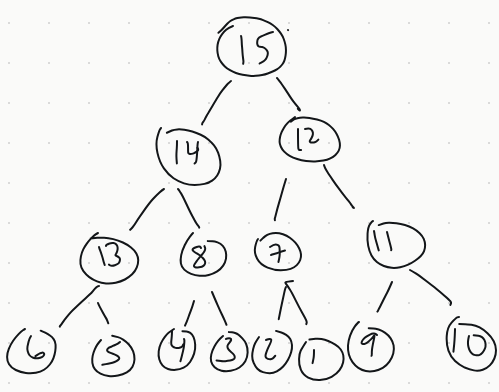
\includegraphics[width=0.5\textwidth]{exercise-14-remove-max-twice}
			\caption{Exercise 14: Heap for which two consecutive \emph{remove the maximum} operations
				would require 6 exchanges.}
			\label{fig:ex-14-remove-max-twice}
		\end{figure}
	\end{sol}
	\begin{ex}{15}
		Design a linear-time certification algorithm to check whether an array \texttt{pq[]}
		is a min-oriented heap.
	\end{ex}
	\begin{sol}
		See \texttt{com.segarciat.algs4.ch2.sec4.MinPQCertification}.
	\end{sol}
	\begin{ex}{17}
		Prove that building a minimum-oriented priority queue of size $k$ then doing
		$n-k$ \emph{replace the minimum} (\emph{insert followed by remove the minimum})
		operation leaves the $k$ largest of the $n$ items in the priority queue.
	\end{ex}
	\begin{sol}
		\begin{proof}
			Suppose the minimum-oriented priority queue has $k$ elements. Suppose
			that the $k$ largest keys are $x_1,\ldots,x_k$, where $x_1$ is the
			largest, and $x_k$ is the $k$th largest.
			
			Let $x_m$ be the $m$th largest, where $m$ is an integer such that $1\leq m\leq k$.
			Then there's at most $m-1$ keys larger than $x_m$, and $m-1<k$. Suppose
			that $x_m$ is already on the priority queue, and a \emph{replace the minimum}
			operation is issued. That is, a new key is added to the queue, so
			that the queue now has $k+1$ keys. Then $x_m$ is not the minimum,
			because if it was, then the other $k$ keys would be larger. But that's
			impossible because at most $m-1<k$ keys are larger than $x_m$. Thus,
			$x_m$ is not eligible for removal, and $x_m$ will remain in the queue.
			Therefore, if one of the $k$ largest keys is already in the queue,
			then it remains in the queue. If $x_m$ is not in the queue, but it is
			inserted, then by the same reasoning, it is not removed from the queue.
			
			Since $m$ is arbitrary with $1\leq m\leq k$, this argument shows that
			$x_1,\ldots,x_k$ all remain in the queue after the $n-k$ operations have
			been issued, because once each goes in the queue, they are never removed.
		\end{proof}
	\end{sol}
	\begin{ex}{18}
		In \texttt{MaxPQ}, suppose that a client calls \texttt{insert()} with an item
		that is larger than all items in the queue, and then immediately calls
		\texttt{delMax()}. Assume that there are no duplicate keys. Is the resulting
		heap identical to the heap as it was before these operations? Answer the
		same for two \texttt{insert()} operations (the first with a key larger
		than all keys in the queue and the second for a key larger than that one)
		followed by two \texttt{delMax()} operations.
	\end{ex}
	\begin{sol}
		For a single \texttt{insert()} and \texttt{delMax()} operation pair, the heap would remain
		the same. Suppose the root is initially $x$, and \texttt{insert()} is called
		with a larger key $y$. Our implementation places $y$ at the end,
		unconditionally swaps it with its parent each time. Let $a_0,a_1,\ldots,a_k$ be
		the sequence of items it is swapped with, where $a_k=x$ . When the \texttt{delMax()}
		operation is issued, $a_0$ is swapped with $y$ before $y$ is removed. Next,
		we \texttt{sink()} starting from $a_0$. We know that $x$ was a child of
		$a_k$, and since that was the largest key before $y$ was added, it is the
		largest key after $y$ is removed. Thus, we swap $a_0$ and $a_k$. Next, $a_k$
		had $a_{k-1}$ as its child, which is now the child of $a_0$. Before $a_{k-1}$
		was swapped down a level, it was larger than its two children, and its old child
		is now the child of $a_0$ (and hence $a_{k-1}$'s sibling). Hence, $a_{k-1}$
		is the largest among the two, so the \texttt{swap()} brings $a_{k-1}$ up a level
		as a child of $a_{k}$. Continuing this way, $a_0$ arrives back at its old location.
		
		I also think the same happens if two \texttt{insert()} operations with larger
		keys each time are then followed by two \texttt{delMax()} operations; the
		resulting heap would be identical.
	\end{sol}
	\begin{ex}{19}
		Implement the constructor for \texttt{MaxPQ} that takes an array of items as
		argument using the bottom-up heap construction method described on page 323
		in the text.
	\end{ex}
	\begin{sol}
		See \texttt{com.segarciat.algs4.ch2.sec4.ex19.MaxPQ}.
	\end{sol}
	\begin{ex}{20}
		Prove that sink-based heap construction uses at most $2n$ compares and $n$
		exchanges.
	\end{ex}
	\begin{proof}
		Suppose that $n=2^k-1$ for some positive integer $k$. Then the heap is
		a perfect binary tree of height $k-1$. At each
		depth $j=0,\ldots,k-1$, there are $2^j$ nodes, so that
		\begin{align*}
			\sum_{j=0}^{k-1}2^j=2^k-1=n
		\end{align*}
		At a depth of $k-1$, a call to \texttt{sink()} would not lead to
		any exchanges because nodes at this depth are leaves. At a depth of $j$,
		a node may only descend through $k-1-j$ levels as a result of \texttt{sink()}.
		At most one exchange may occur then, so that the total number of exchanges
		for the \texttt{sink()} based heap construction is no more than:
		\begin{align*}
			\sum_{j=0}^{k-1}2^{j}\cdot (k-1-j)
			&=k\cdot \sum_{j=0}^{k-1}2^j-\sum_{j=0}^{k-1}2^j
			-\sum_{j=0}^{k-1}j2^j\\
			&=(k-1)(2^k-1)-(k-2)2^k - 2\\
			&=(k-1)(2^k-1)-(k-2)(2^k-1+1)-2\\
			&=2^k-1-(k-2)-2\\
			&=n-k
		\end{align*}
		This confirms the example given during Proposition R, where if we have
		a heap of 127 items, it takes 127 exchanges. This holds because
		$n=127=2^7-1$, so $k=7$, and hence, $120=127-7=n-k$.
	\end{proof}
	I will forego proving the general case.
	\begin{ex}{22}
		\emph{Array resizing}. Add array resizing to \texttt{MaxPQ}, and prove bounds
		like those of Proposition Q for array accesses, in an amortized sense.
	\end{ex}
	\begin{sol}
		I will follow the proof format in Proposition E from Section 1.4:
		\begin{proof}
			For each \texttt{insert()} operation that causes the \texttt{pq}
			array to grow, say from size $n$ to $2n$, consider the $n/2 - 1$
			operations that most recently caused the priority queue (not
			the array) to grow to $k$, for $k$ from size $n/2 +2$ to $n$.
			Each \texttt{insert()} takes about $\sim \lg k$ array accesses.
			The resize from size $n$ to $2n$ takes $4n$ array accesses.
			If we average these operations, we get
			\begin{align*}
				\frac{4n + \sum_{k=n/2}^{n}\lg k}{\sum_{k = \frac{n}{2} + 1}^{n}1}
				&\leq \frac{4n+\lg n!}{n/2}\\
				&\sim \frac{4n+n\lg n}{n / 2}\\
				&=8+\lg n
			\end{align*}
			Here I approximated $\sum_{k=n/2}^{n}\lg k$ as $n\lg n$ using Stirling's
			approximation. Therefore the cost of these $n / 2 - 1$ \texttt{insert()}
			operations is about $\sim \lg n$. Because the remaining operations
			are similarly dependent on the tree depth of the binary heap
			corresponding to the priority queue, the bounds similarly follow.
		\end{proof}
	\end{sol}
	\begin{ex}{24}
		\emph{Priority queue with explicit links}. Implement a priority queue
		using a heap-ordered binary tree, but use a triply linked structure instead
		of an array. You will need three links per node: two to traverse down the
		tree and one to traverse up the tree. Your implementation should guarantee
		logarithmic running time per operation, even if no maximum priority-queue
		size is known ahead of time.
	\end{ex}
	\begin{sol}
		See \texttt{com.segarciat.algs4.ch2.sec4.ex24.LinkedMaxPQ}
	\end{sol}
	\begin{ex}{25}
		\emph{Computational number theory}. Write a program that prints out all integers of
		the form $a^3+b^3$ where $a$ and $b$ are integers between $0$ and $n$ in sorted
		order, without using excessive space. That is, instead of computing an array
		of the $n^2$ sums and sorting them, build a minimum-oriented priority queue,
		initially containing $(0^3, 0, 0), (1^3, 1, 0), (2^3,2,0),\ldots,(n^3,n,n)$.
		Then, while the priority queue is nonempty, \emph{remove the smallest item}
		$(i^3+j^3, i, j)$, print it, and then, if $j < n$, \emph{insert} the item
		$(i^3 + (j+1)^3, i, j+1)$. Use this program to find all distinct integer
		$a$, $b$, $c$, and $d$ between $0$ and $10^6$ such that $a^3+b^3=c^3+d^3$.
	\end{ex}
	\begin{sol}
		See \texttt{com.segarciat.algs4.ch2.sec4.ex25.OrderedSumOfCubes}.
	\end{sol}
	
	\begin{ex}{26}
		\emph{Heap without exchanges}. Because the \texttt{exchange()} primitive is used
		in the \texttt{sink()} and \texttt{swim()} operations, the items are loaded
		and stored twice as often as necessary. Give more efficient implementations
		to avoid this inefficiency, a la insertion sort (see Exercise 2.1.25).
	\end{ex}
	\begin{sol}
		See \texttt{com.segarciat.algs4.ch2.sec4.ex.26.MaxPQ}.
	\end{sol}
	\begin{ex}{27}
		\emph{Find the minimum}. Add a \texttt{min()} method to \texttt{MaxPQ}. Your
		implementation should use constant time and constant extra space.
	\end{ex}
	\begin{sol}
		Simple. We add a private field \texttt{minKey}. On a call to \texttt{insert()},
		we decide if we should update \texttt{minKey} as follows: if the queue
		is empty, then the key we are inserting is the minimum; otherwise, if
		the key being added is smaller, than we update \texttt{minKey} to it.
		On a call to \texttt{delMax()}, we set \texttt{minKey} to \texttt{null}
		if the queue becomes empty, since it would be the last key removed
		from the queue.
	\end{sol}
	\begin{ex}{28}
		\emph{Selection filter}. Write a program similar to \texttt{TopM} that
		reads the points $(x, y, z)$ from standard input, takes a value $m$ from
		the command line, and prints the $m$ points that are closest to the
		origin in Eucledian distance. Estimate the running time of your client
		for $n=10^8$ and $m=10^4$.
	\end{ex}
	\begin{sol}	
		See \texttt{com.segarciat.algs4.ch2.sec4.ex28.ClosestMPoints}.
	\end{sol}
	\begin{ex}{29}
		\emph{Min/max priority queue}. Design a data type that supports the following
		operations: \emph{insert}, \emph{delete the maximum}, and \emph{delete the minimum}
		(all in logarithmic time); and \emph{find the maximum} and \emph{find the minimum}
		(both in constant time). \emph{Hint}: Use two heaps.
	\end{ex}
	\begin{sol}
		See \texttt{com.segarciat.algs4.ch2.sec4.ex29.MinMaxPQ}. I solved this by storing
		all items in both queues. I had to overcome the issue of loitering so
		as to ensure the implementation was garbage-collection friendly.
	\end{sol}
	\begin{ex}{30}
		\emph{Dynamic median-finding}. Design a data type that supports \emph{insert}
		in logarithmic time, \emph{find the median} in constant time, and
		\emph{delete the median} in logarithmic time. \emph{Hint}: Use a min-heap and
		a max-heap.
	\end{ex}
	\begin{sol}
		See \texttt{com.segarciat.algs4.ch2.sec4.ex30.MedianPQ}. I solved this by
		storing the largest half of the items in the min-pq and the smaller half
		of the items in the max-pq. At any time, min-pq was either equal 1 item larger
		than max-pq, and min-pq holds the median as its minimum element. 
	\end{sol}
	\begin{ex}{33}
		\emph{Index priority-queue implementation}. Implement the basic operations in
		the index priority-queue API on page 320, by modifying \textbf{Algorithm 2.6}
		as follows: Change \texttt{pq[]} to hold indices, add an array \texttt{keys[]}
		to hold the key values, and add an array \texttt{qp[]} that is the inverse
		of \texttt{pq[]} --- \texttt{qp[i]} gives the position of \texttt{i} in
		\texttt{pq[]} (the index \texttt{j} such that \texttt{pq[j]} is \texttt{i}).
		Then modify the code in \textbf{Algorithm 2.6} to maintain these data structures.
		Use the convention that \texttt{qp[i] = -1} if \texttt{i} is not on the queue,
		and include a method \texttt{contains()} that tests this condition. You need
		to modify the helper methods \texttt{exchange()} and \texttt{less()}, but
		not \texttt{sink()} and \texttt{swim()}.
	\end{ex}
	\begin{sol}
		See \texttt{com.segarciat.algs4.ch2.sec4.ex33.IndexMinPQ}.
	\end{sol}
	\begin{ex}{34}
		\emph{Index priority-queue implementation (additional operations)}.
		Add \texttt{minIndex()}, \texttt{changeKey()}, and \texttt{delete()}
		to your implementation of \textbf{Exercise 2.4.33}.
	\end{ex}
	\begin{sol}
		See \texttt{com.segarciat.algs4.ch2.sec4.ex34.IndexMinPQ}.
	\end{sol}
	\pagebreak
	\printbibliography
\end{document}